%!TEX root = ../main.tex

\chapter{应用实例——Web新闻聚合系统}

\section{概述}
\label{sec:system-intro}
为了验证本文提出的模板无关的内容抽取技术在爬虫系统中的实际效果,
设计并实现了一个Web新闻聚合系统。
实时采集多种渠道来源的Web新闻,通过模板无关的内容抽取技术抽取新闻正文,
并结合一些领域规则抽取标题、日期等元信息,封装成结构化信息转储在后端的数据仓库中,
提供面向中文的全文检索支持,也为后续的数据分析处理提供了接口。

在这样一个网络信息爆炸的时代,网络舆论对社会的影响越来越重要,
Web新闻聚合系统对关注网络舆情,研究热点事件的产生、传播规律,
构建语料库都具有实际意义。

本章~\ref{sec:system:architecture}~节介绍Web新闻聚合系统的总体架构,
~\ref{sec:system:module}~节详细阐述系统各个模块的设计和关键技术,
~\ref{sec:system:runtime}~节对系统的运行效果进行评估。

\section{系统架构和工作流程}
\label{sec:system:architecture}

\subsection{系统架构}
面对海量异构、持续变化的新闻网站,大数据的存储压力,
在设计Web新闻聚合系统时,需要考虑以下几个关键问题:
\begin{itemize}
\item 关键模块的可扩展能力
\item 存储与检索性能
\item 系统的稳定可用性
\end{itemize}

Web新闻聚合系统的总体架构如图~\ref{fig:architecture}~所示,
标示了系统的关键组件和数据流动情况。

\begin{figure}[htbp]
\centering
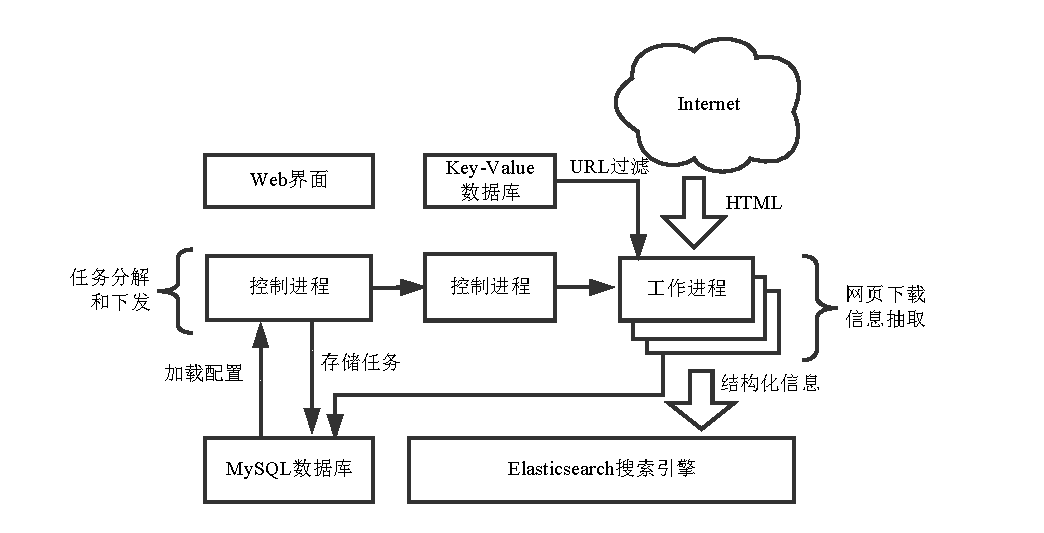
\includegraphics[width=0.9\textwidth]{architecture}
\caption{Web新闻聚合系统整体架构}
\label{fig:architecture}
\end{figure}

\subsection{总体工作流程}
Web新闻聚合系统的核心工作流程分为以下几个部分:

(1)任务分解和下发

MySQL数据库中存储了各个新闻网站的配置,例如RSS源、新闻网页的URL模式等。
Controller作为调度模块,定时从数据库中加载配置,解析并分解为相应任务,
发送到消息队列中,每一条消息都完整包含了完成一个特定任务需要的信息,等待Worker消费并执行。
同时MySQL中还维护了相应的任务表,记录每个任务的基本信息和当前状态。
用户对整个系统的操作都集中在配置中,包括添加新的新闻网站,设定不同的抓取优先级和频率等,
给用户提供了简单统一的接口。

(2)网页下载和信息抽取

网页下载和信息抽取由一组幂等的Worker构成,每个Worker是一个独立的进程,
可以部署在一台机器上,也可以部署在多台机器上进行水平扩展。
Worker监听消息队列,接收任务并执行,根据需要更新数据库或者转发消息给下一个模块。

在新闻采集系统中,任务主要分为两类,新闻列表解析和新闻信息抽取。
新闻列表解析就是从RSS源或包含新闻列表的网页中,抽取每一篇新闻的URL,供后续信息抽取。
然后新闻信息抽取模块根据指定的URL,抽取新闻正文和标题等元信息,然后转储在数据仓库中。
为了防止重复抓取同一个页面而造成资源浪费,还需要一个全局的URL过滤组件,
判断当前URL是否已经重复,这里使用Redis实现。

(3)存储与检索

MySQL作为传统的关系型数据库,不擅长全文检索,
因此选用了Elasticsearch作为存储和检索引擎,将需要检索支持的结构化信息导入Elasticsearch,
而把传统的配置管理、任务管理等交给MySQL处理,充分发挥各自的优势。
Elasticsearch具有很强的扩展能力,多机部署构成集群,面向用户提供透明的HTTP接口,
能够满足存储和检索的分布式扩展需求。

\subsection{新闻采集流程}
Web新闻从多种信息来源采集,对每一个新闻来源,系统都有与之对应的新闻列表解析模块,
从不同渠道的来源中解析新闻页面URL,转交给信息抽取模块。
这种架构的优势在于,通过消息队列的中转,新闻列表解析和新闻信息抽取相互解耦,
屏蔽底层细节,为信息抽取提供统一的接口,也利于计算资源的水平扩展。

图~\ref{fig:architecture}~表现了Controller和Worker的一般关系,
为了详细阐述新闻采集过程,将Worker细分为负责新闻列表解析的Parser,
以及负责新闻信息抽取的Extractor,形成图~\ref{fig:crawler}~。
其中1--6标示的是各个流程:
\begin{enumerate}
\item Controller以定时任务或其它方式触发,从MySQL数据库加载配置;
\item Controller分解任务,封装为消息投放到消息队列中,
消息还可以设定相应的优先级和延迟执行时间,从而灵活配置计算资源;
\item Parser接收任务后从指定的新闻源解析得到一系列新闻URL;
\item Parser将新闻URL封装成消息投放到消息队列中;
\item Extractor接收任务后从URL指定的新闻页面中,抽取正文内容及其它元信息;
\item Extractor将新闻正文内容及其它元信息转储到Elasticsearch中;
\end{enumerate}

\begin{figure}[htbp]
\centering
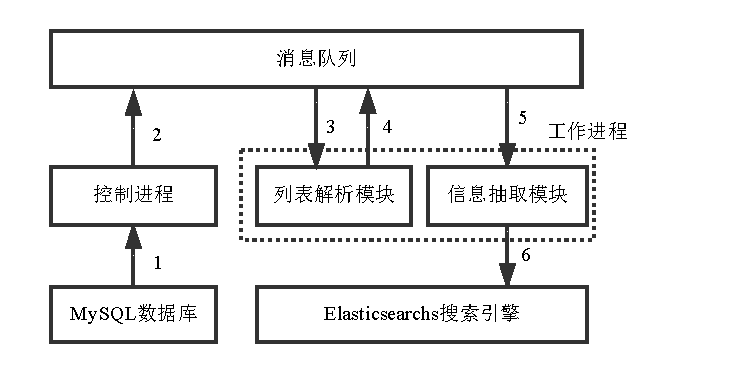
\includegraphics[width=0.9\textwidth]{crawler}
\caption{新闻采集流程}
\label{fig:crawler}
\end{figure}

\section{系统模块和关键技术}
\label{sec:system:module}

\subsection{新闻列表解析}
Web新闻采集的来源包括RSS、元搜索和一般新闻网站三类。
RSS是被广泛接受的标准信息聚合接口,这是系统优先考虑的采集来源,
但部分新闻网站可能不提供RSS接口,所以需要针对一般新闻网站的列表解析模块。
元搜索利用现有搜索引擎对新闻的聚合能力,是对热点新闻聚合的一种补充方式。

\subsubsection{RSS}
RSS可以是以下三个解释的其中一个:
\begin{itemize}
\item Really Simple Syndication
\item RDF (Resource Description Framework) Site Summary
\item Rich Site Summary
\end{itemize}

RSS使用一组标准的Web信息流格式来发布频繁更新的信息,如博客、新闻头条和音视频等。
RSS是互联网上被广泛采用的内容包装和投递协议,搭建了一个信息迅速传播的技术平台,
使得每个人都成为潜在的信息提供者。

一个RSS文档包含摘要内容和一些元信息,例如发布日期和作者的名字。
RSS是XML格式的普通文本,简单的格式使得它既能被程序自动化解析也能被普通人理解,
一个RSS如例~\ref{ex:rss}~所示\footnote{https://en.wikipedia.org/wiki/RSS}。

\begin{figure}[t]
\begin{example}
\label{ex:rss}
RSS示例
\end{example}
\begin{verbatim}
<?xml version="1.0" encoding="UTF-8" ?>
<rss version="2.0">
<channel>
  <title>RSS Title</title>
  <description>This is an example of an RSS feed</description>
  <link>http://www.example.com/main.html</link>
  <lastBuildDate>Mon, 06 Sep 2010 00:01:00 +0000 </lastBuildDate>
  <pubDate>Sun, 06 Sep 2009 16:20:00 +0000</pubDate>
  <ttl>1800</ttl>

  <item>
    <title>Example entry</title>
    <description>Here is an interesting description.</description>
    <link>http://www.example.com/blog/post/1</link>
    <guid isPermaLink="true">7bd204c6-1655-4c27</guid>
    <pubDate>Sun, 06 Sep 2009 16:20:00 +0000</pubDate>
 </item>
</channel>
</rss>
\end{verbatim}
\end{figure}

在新闻列表解析模块,我们最关心的是新闻页面的URL,即\texttt{<link>}。
通过简单的正则表达式匹配,就能抽取出一组新闻页面的URL,然后提交给新闻信息抽取模块。

\subsubsection{元搜索}
为了利用现有搜索引擎对新闻的聚合能力,系统还采用元搜索的方式获得新闻。
元件搜索引擎又称集合型搜索引擎,将多个单一搜索引擎集成在一起,
将用户的检索提问同时提交给多个独立的搜索引擎,同时检索多个数据库。
并根据多个独立搜索引擎的检索结果进行二次加工,如对检索结果去重、排序,然后输出给自己。

元搜索根据关键词提交查询请求,系统通过维护热点关键词列表,能够及时获得热点新闻,
这对于热点新闻的聚合是一种有效的补充方式。
Web新闻聚合系统面向国内舆情热点,选取了知名的中文搜索引擎百度
\footnote{http://www.baidu.com/}和360\footnote{https://www.so.com/}
作为元搜索入口:
\begin{itemize}
\item http://news.baidu.com/ns?word=\textbf{keyword}\&tn=news\&from=news
\item http://news.so.com/ns?q=\textbf{keyword}\&src=newhome
\end{itemize}

URL中粗体标示的\textbf{keyword}可以替换为搜索关键词,搜索引擎会返回与之相关的新闻。
如图~\ref{fig:baidu}~所示的百度新闻搜索,包含了新闻题目、摘要、发布时间和链接等信息。
通过人工编写的包装器,可以抽取出一组新闻页面的URL,
由于搜索引擎较少,编写包装器的开销并不大。

\begin{figure}[htbp]
\centering
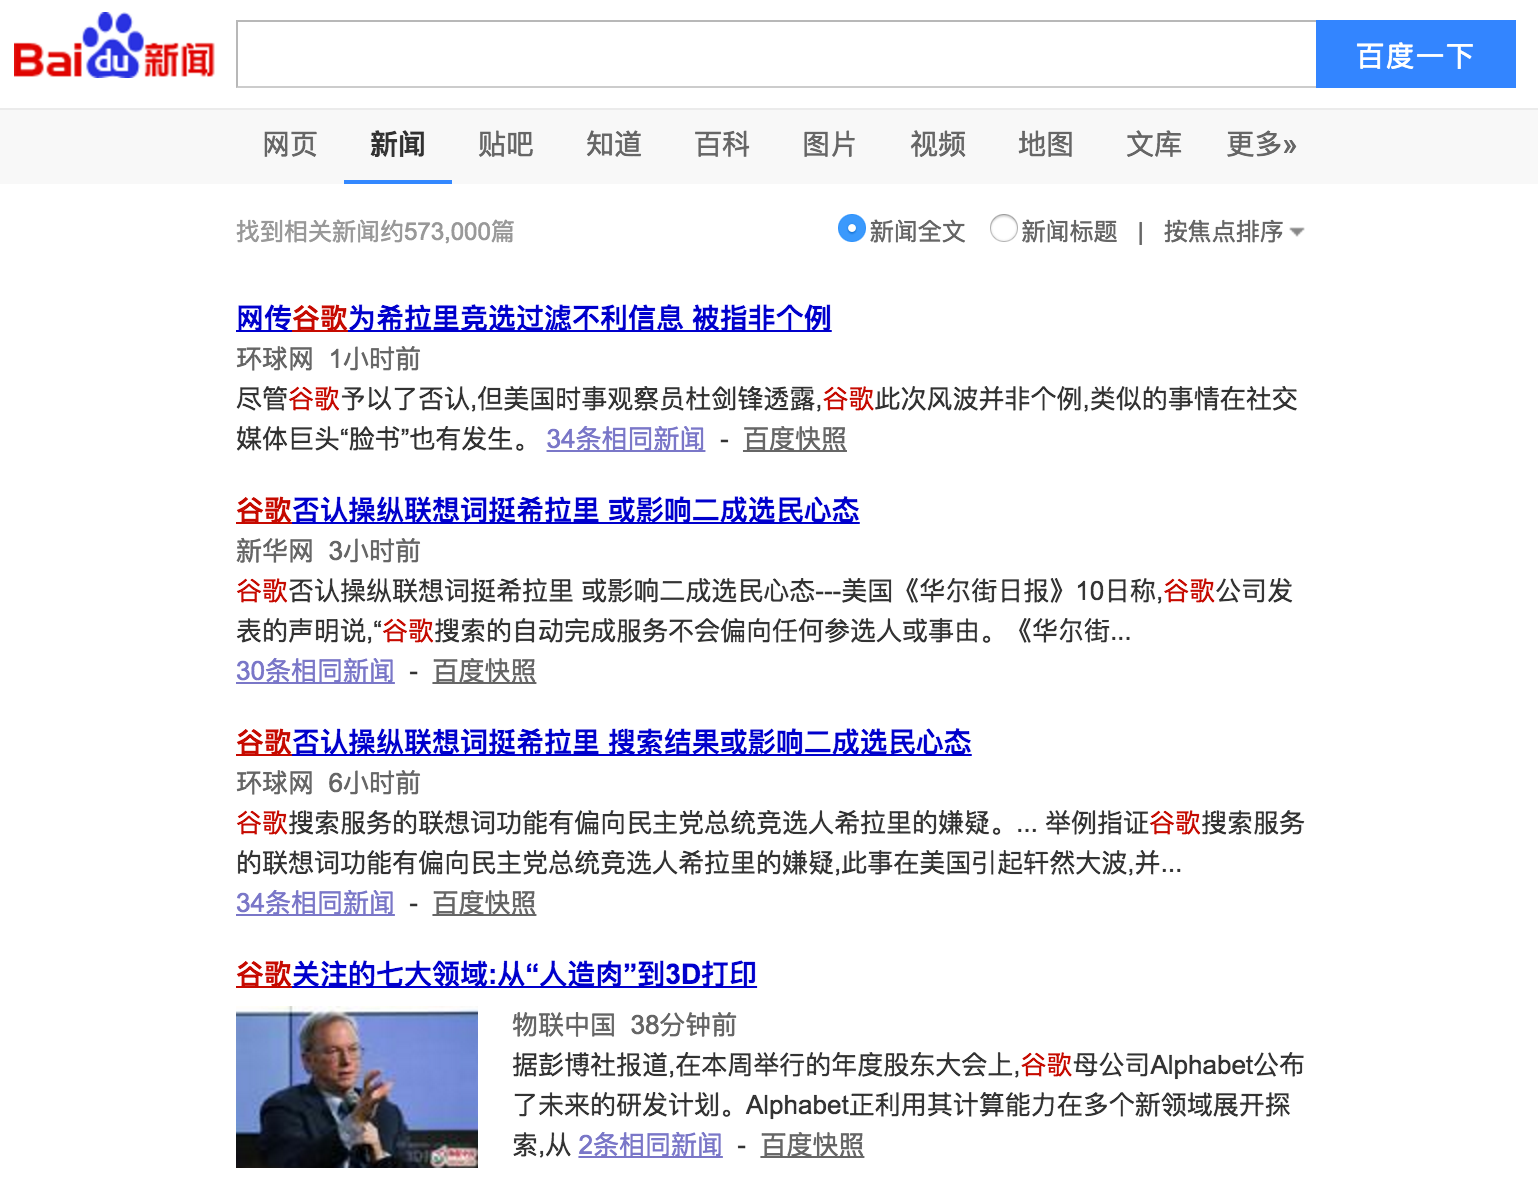
\includegraphics[width=0.9\textwidth]{baidu}
\caption{百度新闻搜索}
\label{fig:baidu}
\end{figure}

\subsubsection{一般新闻网站}
RSS基于XML提供了一种统一的信息发布格式,大大降低了聚合信息的代价,
也是系统优先考虑的采集来源。
但仍存在部分新闻网站,不提供RSS接口,我们采用编写包装器的方式解析新闻列表。
因为我们关心的是新闻页面的URL,所以包装器主要包含新闻页面URL的正则表达式。

如表~\ref{tbl:url-pattern}~所示,这是一组新闻页面URL的正则表达式,
其中既包含绝对地址(\verb|http://\w+.cnr.cn/\w+/\w+/\d{8}/\w+.shtml|),
也包含相对地址(\verb|/news/\w+/story\d+-\d+|)。
在新闻列表的HTML页面上匹配相应的URL模式,再根据相对地址、绝对地址进行转换,
就能抽取出一组新闻页面的URL。

\begin{table}[htbp]
\caption{新闻页面URL模式}
\label{tbl:url-pattern}
\vspace{0.5em}\centering\wuhao
\begin{tabular}{lll}
\toprule[1.5pt]
编号 & 新闻网站 & URL模式 \\
\midrule[1pt]
1 & 联合早报 & \verb|/news/\w+/story\d+-\d+| \\
2 & 中国信息网 & \verb|/\w+/\d\d\d\d/\d\d-\d\d/\d+.shtml| \\
3 & 南方网 & \verb|http://\w+.southcn.com/\w+/\d\d\d\d-\d\d/\d\d/content_\d+.htm| \\
4 & 央广网 & \verb|http://\w+.cnr.cn/\w+/\w+/\d{8}/\w+.shtml| \\
5 & 中国军网 & \verb|\d\d\d\d-\d\d/\d\d/content_\d+.htm| \\
\bottomrule[1.5pt]
\end{tabular}
\end{table}

\subsection{新闻信息抽取}
新闻信息抽取模块的输入是新闻页面的URL,然后返回抽取的发布日期、标题和新闻正文三元组。
新闻信息抽取流程如图~\ref{fig:news-extract}~所示,在抽取各项信息之前,
还需要检测新闻网页的编码格式,将HTML文档在内存中解析为DOM树。
在信息抽取结束后,还需要判断抽取的三元组是否有效,无效则放弃。

\begin{figure}[htbp]
\centering
\begin{tikzpicture}[node distance = 2cm, auto]
\node[startstop](init){开始};
\node[io, below of=init](input){新闻URL};
\node[process, below of=input](encoding){编码格式检测};
\node[process, below of=encoding](DOM){DOM树解析};
\node[process, right of=init, xshift=3cm](date){发布日期抽取};
\node[process, below of=date](title){标题抽取};
\node[process, below of=title](content){新闻正文抽取};
\node[decision, below of=content, yshift=-0.5cm](verify){是否有效?};
\node[io, below of=verify, yshift=-0.5cm](output){日期,标题,正文};
\node[startstop, below of=output](stop){结束};
\node[startstop, right of=verify, xshift=3cm](failed){失败};

\draw[arrow](init)--(input);
\draw[arrow](input)--(encoding);
\draw[arrow](encoding)--(DOM);
\draw[thick,->] (DOM) -| ++(2,0) |- (date);
\draw[arrow](date)--(title);
\draw[arrow](title)--(content);
\draw[arrow](content)--(verify);
\draw[arrow](verify)--node[near start]{是}(output);
\draw[arrow](verify)--node[near start]{否}(failed); 
\draw[arrow](output)--(stop);
\end{tikzpicture}
\caption{新闻信息抽取流程图}
\label{fig:news-extract}
\end{figure}

\subsubsection{发布日期}
发布日期是构成新闻必不可少的元素,新闻的发布日期一般在标题之下。
通过~\ref{subsec:anchor}~节中提供的日期正则表达式,
可以从HTML文档中抽取日期,从中进行筛选得到最终的发布日期。
发布日期的抽取过程如算法~\ref{algo:extract-date}~所示,
只选择大于某个特定时期(如2016年1月1日),并且在当前时间之前的日期作为候选,
最后从其中选择最近的日期,作为这篇新闻的发布日期。

\begin{algorithm}[htbp]
\caption{extractPubDate(Src)}
\label{algo:extract-date}
\KwIn{HTML Text Src}
\KwOut{Publication date}

candidate\_dates = $\emptyset$ \;
\For{every date string $s$ extracted from Src via regular expression}{
  Build date structure $d$ from date string $s$ \;
  \If{$d$ > 2016/1/1 \textbf{and} $d$ < now()}{
    candidate\_dates.add($d$) \;
  }
}
\eIf{candidate\_dates is not null}{
  \Return maximum(candidate\_dates) \;
}{
  \Return null \; 
}
\end{algorithm}

\subsubsection{新闻标题}
HTML文档中\texttt{<title>}标签表示网页的标题,但它一般不能直接作为新闻的标题。
以~\ref{sec:cevc-intro}~节图~\ref{fig:news}~为例,
这篇新闻的\texttt{<title>}为
\textbf{国务院参事:“建10个类似北京超大城市”是误解|仇保兴|超大城市\_新浪新闻},
但其中包含了分隔符、关键词、新闻网站名称,需要从中过滤这些额外信息。
通过观察发现,新闻的标题一般也会出现在HTML文档的\texttt{<h1>}标签中,
\texttt{<h1>}表示一级标题。
在计算\texttt{<titie>}和\texttt{<h1>}的最长公共子串后,这些额外信息就能被过滤。

为了新闻标题抽取的准确性,我们通过以下步骤确定最终的标题:
\begin{enumerate}
\item 抽取\texttt{<title>}和\texttt{<h1>};
\item 计算\texttt{<titie>}和\texttt{<h1>}的最长公共子串;
\item 如果最长公共子串长度小于5,选取\texttt{<titie>}为标题;
\item 如果\texttt{<titie>}为空,选取\texttt{<h1>}为标题。
\end{enumerate}

\subsubsection{新闻正文}
根据~\ref{sec:cevc-experiment}~节的对比结果,我们选择本文提出的
CEVC(Content Extraction via Valid Characters)算法来抽取新闻正文。
CEVC易于实现,预处理阶段依赖小,并且在多个数据集上得到了优于其它对比算法的抽取结果。

\subsection{存储和检索}
由于传统的关系型数据库MySQL对中文全文检索支持不足,且扩展性差,
除了配置管理、任务管理等传统业务存储于MySQL中,
未来增长较快、关系结构简单、需要全文检索的数据则存储于其它数据仓库中。

在对比了Mongodb\footnote{https://www.mongodb.com/},
Solr\footnote{http://lucene.apache.org/solr/}和
Elasticsearch\footnote{https://www.elastic.co/}后,
我们选择了Elasticsearch作为数据存储和检索的一体化平台。

Elasticsearch是一个实时的分布式搜索和分析引擎,
它建立在全文搜索引擎框架Apache Lucence\footnote{http://lucene.apache.org/}
的基础之上,其诞生伊始就完全基于分布式架构。
Elasticsearch可以用于全文搜索、结构化搜索和分析,
在当前互联网上已经有许多成功使用的案例:
\begin{itemize}
\item Github使用Elasticsearch搜索20TB的数据,
包括13亿的文件和1300亿行的代码\citeup{paro2015elasticsearch};
\item Stackoverflow使用Elasticsearch代替SQL全排索引,因为其良好的扩展性和低成本;
\item 维基百科使用Elasticsearch进行全文检索并高亮显示搜索关键词;
\end{itemize}

Elasticsearch为了提供一个扩展性强同时易用的分布式系统,做了许多自动化工作,
例如文档划分到不同容器或者分片中,集群中索引和搜索的跨节点负载均衡,
数据分片的自动冗余备份,无缝扩展或者恢复整个集群。

Elasticsearch是面向文档的分布式搜索引擎,文档可以代表一个对象。
新闻对象在Elasticsearch中的字段映射如例~\ref{ex:news-mapping}~所示,
其中定义了\texttt{pubdate}为日期类型,\texttt{title}和\texttt{content}为字符串,
\texttt{smartcn}是所使用的中文分词组件。

\begin{figure}[t]
\begin{example}
\label{ex:news-mapping}
新闻对象的字段映射
\end{example}
\begin{verbatim}
"news": {
  "properties": {
    "url": {"type": "string"},
    "src": {"type": "string"},
    "pubdate": {"type": "date", "format": "yyyy-MM-dd HH:mm:ss"},
    "title": {"type": "string", "analyzer": "smartcn"},
    "content": {"type": "string", "analyzer": "smartcn"}
  }
}
\end{verbatim}
\end{figure}

\section{运行效果评估}
\label{sec:system:runtime}

Web新闻聚合系统的开发环境是一台MacBook Pro(2 GHz Intel Core i7处理器,
8G内存,256G SSD),系统功能的实现得益于许多开源项目的支持:
\begin{itemize}
\item 编程语言:Python 2.7
\item 存储与检索:MySQL,Elasticsearch,Redis
\item 消息队列:Beanstalkd
\item Web:Flask Web Framework,JQuery,Bootstrap
\end{itemize}

\newcommand{\slice}[4]{
  \pgfmathparse{0.5*#1+0.5*#2}
  \let\midangle\pgfmathresult

  % slice
  \draw[thick,fill=black!10] (0,0) -- (#1:1) arc (#1:#2:1) -- cycle;

  % outer label
  \node[label=\midangle:#4] at (\midangle:1) {};

  % inner label
  \pgfmathparse{min((#2-#1-10)/110*(-0.3),0)}
  \let\temp\pgfmathresult
  \pgfmathparse{max(\temp,-0.5) + 0.8}
  \let\innerpos\pgfmathresult
  \node at (\midangle:\innerpos) {#3};
}

\begin{figure}[htbp]
\centering
\begin{tikzpicture}[scale=3]
\newcounter{a}
\newcounter{b}
\foreach \p/\t in {
15/中国新闻网,
13/环球网,
10/南方网,
10/新华网,
10/凤凰资讯,
42/其它
}{
  \setcounter{a}{\value{b}}
  \addtocounter{b}{\p}
  \slice{\thea/100*360}
        {\theb/100*360}
        {\p\%}{\t}
}

\end{tikzpicture}
\caption{新闻网站的采集情况}
\label{fig:news-breakdown}
\end{figure}

系统从2016年6月8日至14日,平均每天采集2000条新闻,
涉及政治、经济和时事等各个方面。
新闻数量TOP 5的网站分布如图~\ref{fig:news-breakdown}~所示,
新闻采集量最多的网站依次是中国新闻网、环球网、南方网、新华网和凤凰资讯。

为了评估新闻信息抽取模块对标题、发布日期抽取的准确率,
我们从系统采集的新闻中随机抽取200篇,人工审核标题、发布日期抽取是否正确,
最终结果如表~\ref{tbl:title-date}~所示。
新闻标题通过\texttt{<title>}和\texttt{<h1>}联合确定,
在新闻网页中基本都符合这个规律,所以在样本中准确率达到了100\%。
而发布日期的判断不够严谨,可能被网页中的其它日期干扰,影响了最终的准确率。

需要注意的是,新闻信息抽取模块在抽取标题、发布日期和新闻内容三元组后,
进行了简单的有效性判断(标题多于5个字,发布日期有效,新闻内容多于100个字)。
这使得系统在采集过程中,丢弃了部分新闻,可能是由于正当的原因(URL失效,非新闻网页),
也可能由于信息抽取的失败,所以表~\ref{tbl:title-date}~中的结果要优于实际情况。

\begin{table}[htbp]
\caption{新闻标题和发布日期抽取效果评估}
\label{tbl:title-date}
\vspace{0.5em}\centering\wuhao
\begin{tabular}{llll}
\toprule[1.5pt]
抽取项目 & 总数量 & 正确数量 & 准确率 \\
\midrule[1pt]
标题 & 200 & 200 & 100\% \\
发布日期 & 200 & 191 & 95.5\% \\  
标题和发布日期 & 200 & 191 & 95.5\% \\
\bottomrule[1.5pt]
\end{tabular}
\end{table}

新闻检索界面如图~\ref{fig:web-ui}~所示,
在检索框输入关键词“奥兰多”,系统返回与之关联的新闻,并对关键词进行高亮处理。
表格中只给出了新闻内容的部分片段,点击新闻标题,
能够进入一个独立的页面,详细展示全部新闻内容。
借助于Elasticsearch,系统能够从数据仓库中匹配标题或正文包含搜索关键词的新闻,
并按照相关性的高低排序返回结果。
Elasticsearch使用了高效的索引结构,系统对关键词查询的响应时间在0.5秒以内,
能够适应实时检索的要求。

Web新闻聚合系统使用了模板无关的内容抽取算法CEVC,
并结合一些领域规则抽取标题、发布日期,
不需要对新闻页面单独构造包装器,大大降低了系统扩展和维护的成本。

系统从RSS、元搜索和一般新闻网站三个信息来源采集新闻,
通过模板无关的抽取技术整合了各个渠道的差异,使人工成本限制在新闻列表解析中。
借助于RSS的统一协议和元搜索技术,新闻列表解析中人工配置和包装器构造的成本能够接受。
系统的后续工作将集中于如何自动扩展新闻采集来源,进一步降低人工参与的成本,
实现系统的高度自动化。

\begin{figure}[htbp]
\centering
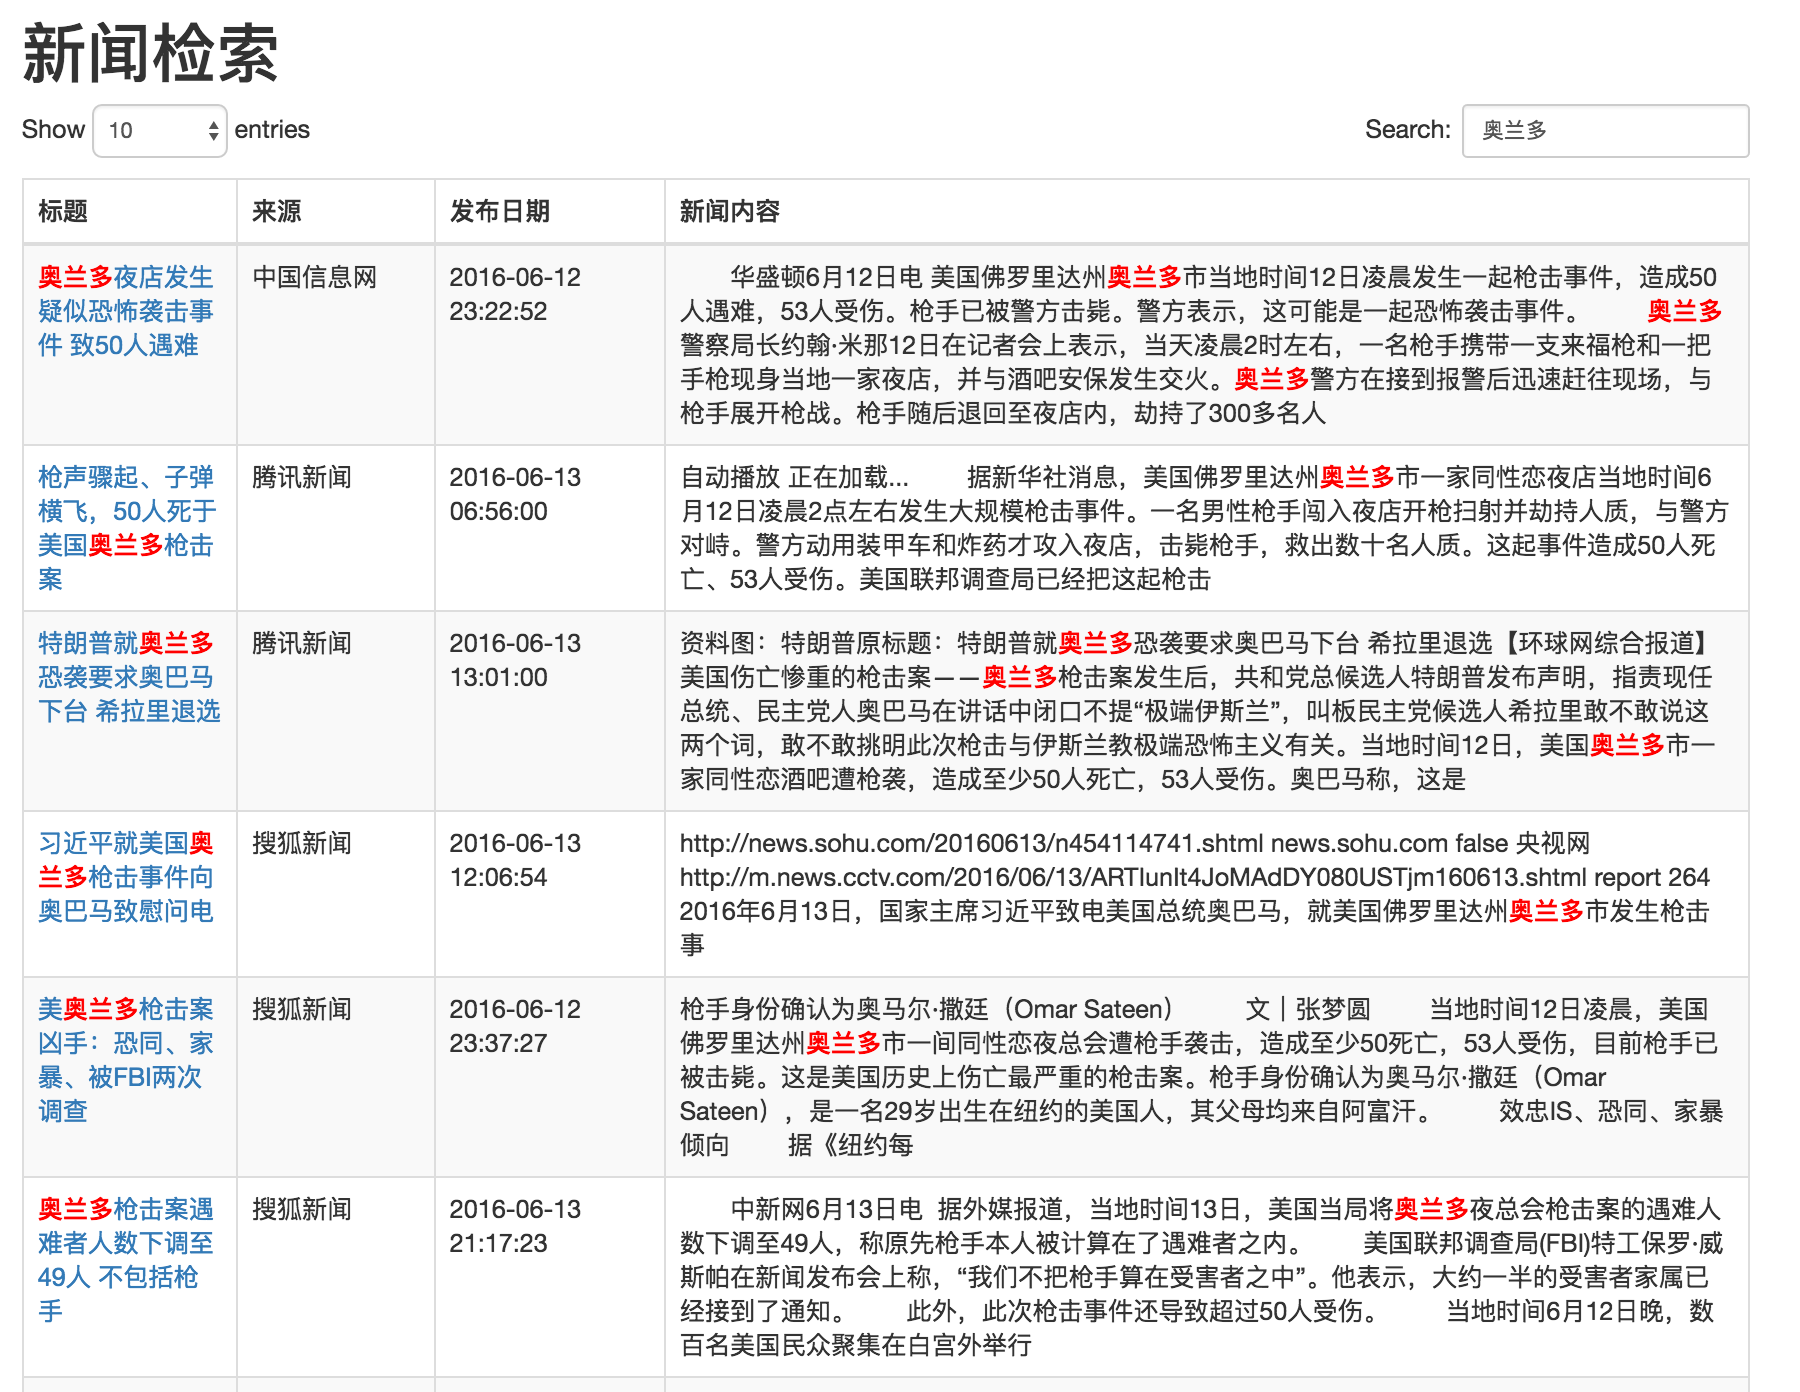
\includegraphics[width=0.9\textwidth]{web-ui}
\caption{新闻检索界面}
\label{fig:web-ui}
\end{figure}
